\documentclass[a4paper,twocolumn,11pt]{ltjsarticle}
\usepackage[no-math,deluxe,expert]{luatexja-preset}
\usepackage{setspace}
\usepackage{fun-report-template}
\setstretch{0.8}
\parindent = 0pt

\course{データの可視化}
\title{バス乗降データの可視化}
\class{3-B}
\id{1022237}
\author{寸田和輝}
\date{\today}

\setmainjfont{A P-OTF Shuei5+ ProN R}
\setsansjfont{ShinGoPr6-Medium}

\begin{document}

\maketitle

\section{可視化結果について}

\begin{figure*}[b]
    \centering
    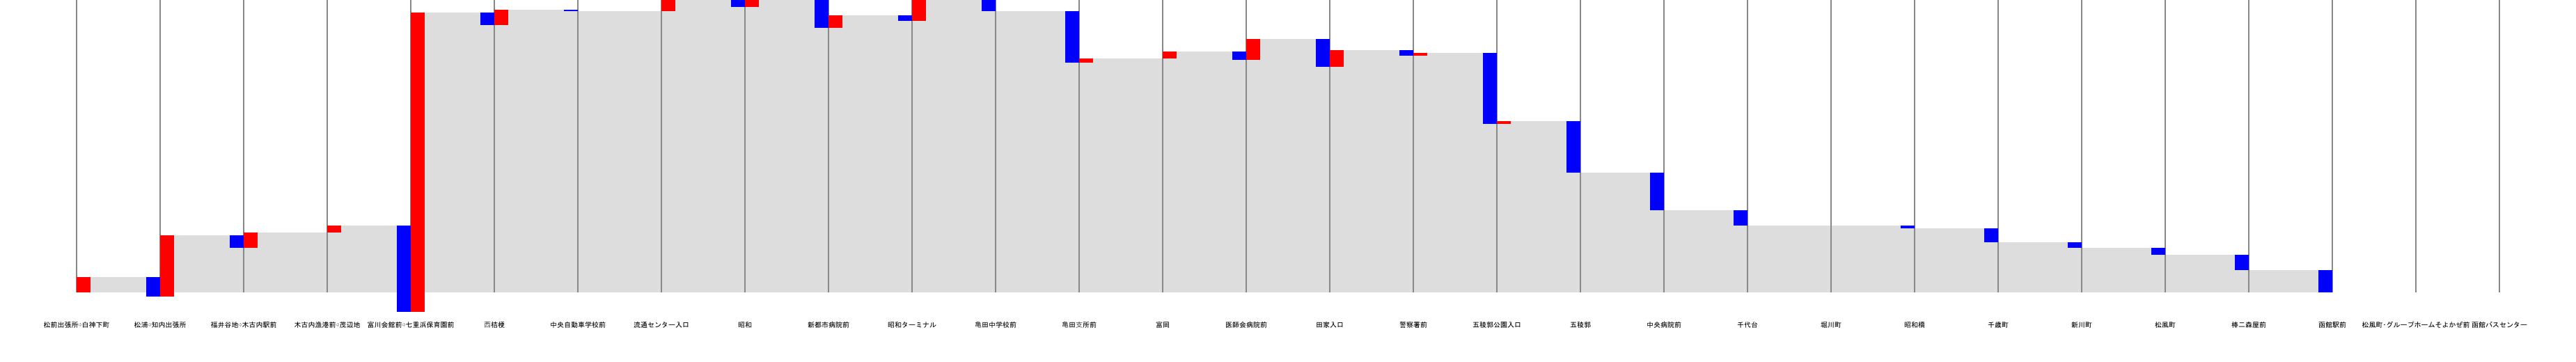
\includegraphics[width=16cm]{visualize.png}
    \caption{可視化されたバス乗降客数データの例}
    \label{fig:dvz}
\end{figure*}

510・511系統 松前出張所~函館バスセンター 停留所別乗降実績表(平日)の可視化に取り組んだ。
図\ref{fig:dvz}に示されるような可視化を行った。可視化の種類は、棒グラフとサンキー図の融合のようなものだと考えられるが、既存の可視化とは完全に一致するものは、授業では取り上げられていなかった。
詳しいものは\url{https://dvz.jugesuke.net/}で確認できる。
青色のバーが降車数、赤色のバーが乗車数、左右に伸びる灰色のバーが各駅間の利用客数を表している。
この可視化は、Reactを用いて乗降データを加工したものをもとにsvgを自動で生成し、作成した\footnote{\url{https://github.com/jugesuke/dvz24-ex}}。
このデータは、令和6年度第4回 函館市地域公共交通協議会総会 (資料2)バス路線の系統廃止および路線廃止について\footnote{\url{https://www.city.hakodate.hokkaido.jp/docs/2024051300054/} CC-BY-NC 函館市} に掲載のデータを使用した。

この資料に掲載されているのは、停留所ごとの乗車・降車・通過\footnote{ここでいう通過は乗車人員を含めているようである}の人数が表形式で掲載されているが、ここからは、どのような傾向があるのかを読み取ることは困難である。

\section{可視化からわかること}

このデータを可視化したことで、以下のことが確認できる。

\begin{itemize}
    \item 各停留所間における利用客の数
    \item 各停留所における乗降の激しさ
    \item 区間別の利用客の差
\end{itemize}

函館駅方面においては、富川会館前⇨七重浜保育園前から五稜郭付近に利用が集中している。
松前出張所方面においては、五稜郭から七重浜保育園前⇨富川会館前に利用が集中している。
また、亀田支所前においては乗降が激しく行われていることが読み取れる。
加えて、函館バスセンター 16:42発のバスについては、木古内本町⇨知内元町から知内公園入口⇨松浦にかけて突出して利用されていることがわかる。
可視化結果から、富川会館前~松前出張所・富川会館前~五稜郭・五稜郭~函館バスセンターで利用が大きく分かれていることがわかった。

データからは、どこが具体的に利用が多いのかなどはとてもわかりにくかったが、可視化によって一目でわかるようになった。

\section{可視化からはわからないこと}

可視化からわからないこととして、以下のことが挙げられる。

\begin{itemize}
    \item 具体的な乗車人数
    \item バスの混雑状況
    \item まとめられてしまっている区間の具体的な乗降客数
\end{itemize}

グラフにしたことで、具体的に何人なのかがわからなくなってしまった。
また、グラフの高さの程度がわかりにくくなっている。
バス定員に対する割合を表示することでより分かりやすくなるように感じる。
しかし、バス定員は運行する車両によって異なるので、函館バスで運行しているバスの平均などを表示するよよいと考えた。
また、データでは、一部区間がまとめられて掲載されている。そのため、その区間の乗降はわからない。加えて、この区間においては実際に通過した人数はわからなくなってしまっている。

\end{document}
